
\bta{2005}




\section{Use of English}

\noindent
\textbf{Directions:}\\
{Read the following text. Choose the best word (s) for each
	numbered blank and mark A, B, C or D on ANSWER
	SHEET 1. (10 points)


\TiGanSpace


The human nose is an underrated tool. Humans are often thought to be
insensitive smellers compared with animals, \cloze this is
largely because, \cloze animals, we stand upright. This means that
our noses are \cloze to perceiving those smells which float
through the air, \cloze the majority of smells which stick to
surfaces. In fact, \cloze , we are extremely sensitive to
smells, \cloze we do not generally realize it. Our noses are
capable of \cloze human smells even when these
are \cloze to far below one part in one million.

Strangely, some people find that they can smell one type of flower but
not another, \cloze others are sensitive to the smells of both
flowers. This may be because some people do not have the genes necessary
to generate \cloze smell receptors in the nose. These receptors
are the cells which sense smells and send \cloze to the brain.
However, it has been found that even people insensitive to a certain
smell \cloze can suddenly become sensitive to it
when \cloze to it often enough.

The explanation for insensitivity to smell seems to be that brain finds
it \cloze to keep all smell receptors working all the time but
can \cloze new receptors if necessary. This
may \cloze explain why we are not usually sensitive to our own
smells---we simply do not need to be. We are not \cloze of the
usual smell of our own house, but we \cloze new smells when we
visit someone else's. The brain finds it best to keep smell
receptors \cloze for unfamiliar and emergency
signals \cloze the smell of smoke, which might indicate the
danger of fire.


\newpage

\begin{enumerate}
	%\renewcommand{\labelenumi}{\arabic{enumi}.}
	% A(\Alph) a(\alph) I(\Roman) i(\roman) 1(\arabic)
	%设定全局标号series=example	%引用全局变量resume=example
	%[topsep=-0.3em,parsep=-0.3em,itemsep=-0.3em,partopsep=-0.3em]
	%可使用leftmargin调整列表环境左边的空白长度 [leftmargin=0em]
	\item


\fourchoices
{although}
{as}
{but}
{while}




\item


\fourchoices
{above}
{unlike}
{excluding}
{besides}




\item


\fourchoices
{limited}
{committed}
{dedicated}
{confined}




\item


\fourchoices
{catching}
{ignoring}
{missing}
{tracking}




\item


\fourchoices
{anyway}
{though}
{instead}
{therefore}




\item


\fourchoices
{even if}
{if only}
{only if}
{as if}




\item

\fourchoices
{distinguishing}
{discovering}
{determining}
{detecting}


\item


\fourchoices
{diluted}
{dissolved}
{dispersed}
{diffused}




\item


\fourchoices
{when}
{since}
{for}
{whereas}




\item


\fourchoices
{unusual}
{particular}
{unique}
{typical}




\item


\fourchoices
{signs}
{stimuli}
{messages}
{impulses}




\item


\fourchoices
{at first}
{at all}
{at large}
{at times}




\item


\fourchoices
{subjected}
{left}
{drawn}
{exposed}




\item

\fourchoices
{ineffective}
{incompetent}
{inefficient}
{insufficient}


\item


\fourchoices
{introduce}
{summon}
{trigger}
{create}




\item


\fourchoices
{still}
{also}
{otherwise}
{nevertheless}




\item


\fourchoices
{sure}
{sick}
{aware}
{tired}




\item


\fourchoices
{tolerate}
{repel}
{neglect}
{notice}




\item

\fourchoices
{available}
{reliable}
{identifiable}
{suitable}


\item


\fourchoices
{similar to}
{such as}
{along with}
{aside from}



\end{enumerate}

\vfil

\section{Reading Comprehension}


\noindent
\textbf{Part A}\\
\textbf{Directions:}\\
Read the following four texts. Answer the questions below each
	text by choosing A, B, C or
	D. Mark your answers
	on ANSWER SHEET 1. (40 points)

\newpage
\subsection{Text 1}


Everybody loves a fat pay rise. Yet pleasure at your own can vanish if
you learn that a colleague has been given a bigger one. Indeed, if he
has a reputation for slacking, you might even be outraged. Such
behaviour is regarded as ``all too human'', with the underlying
assumption that other animals would not be capable of this finely
developed sense of grievance. But a study by Sarah Brosnan and Frans de
Waal of Emory University in Atlanta, Georgia, which has just been
published in \emph{Nature}, suggests that  \emph{it is all too monkey}, as well.

The researchers studied the behaviour of female brown capuchin monkeys.
They look cute. They are good-natured, co-operative creatures, and they
share their food readily. Above all, like their female human
counterparts, they tend to pay much closer attention to the value of
``goods and services'' than males.

Such characteristics make them perfect candidates for Dr. Brosnan's and
Dr. de Waal's study. The researchers spent two years teaching their
monkeys to exchange tokens for food. Normally, the monkeys were happy
enough to exchange pieces of rock for slices of cucumber. However, when
two monkeys were placed in separate but adjoining chambers, so that each
could observe what the other was getting in return for its rock, their
behaviour became markedly different.

In the world of capuchins grapes are luxury goods (and much preferable
to cucumbers). So when one monkey was handed a grape in exchange for her
token, the second was reluctant to hand hers over for a mere piece of
cucumber. And if one received a grape without having to provide her
token in exchange at all, the other either tossed her own token at the
researcher or out of the chamber, or refused to accept the slice of
cucumber. Indeed, the mere presence of a grape in the other chamber
(without an actual monkey to eat it) was enough to induce resentment in
a female capuchin.

The researchers suggest that capuchin monkeys, like humans, are guided
by social emotions. In the wild, they are a co-operative, group-living
species. Such co-operation is likely to be stable only when each animal
feels it is not being cheated. Feelings of righteous indignation, it
seems, are not the preserve of people alone. Refusing a lesser reward
completely makes these feelings abundantly clear to other members of the
group. However, whether such a sense of fairness evolved independently
in capuchins and humans, or whether it stems from the common ancestor
that the species had 35 million years ago, is, as yet, an unanswered
question.

\begin{enumerate}[resume]
	%\renewcommand{\labelenumi}{\arabic{enumi}.}
	% A(\Alph) a(\alph) I(\Roman) i(\roman) 1(\arabic)
	%设定全局标号series=example	%引用全局变量resume=example
	%[topsep=-0.3em,parsep=-0.3em,itemsep=-0.3em,partopsep=-0.3em]
	%可使用leftmargin调整列表环境左边的空白长度 [leftmargin=0em]
	\item
In the opening paragraph, the author introduces his topic by \lineread.


\fourchoices
{posing a contrast}
{justifying an assumption}
{making a comparison}
{explaining a phenomenon}


\item
The statement ``it is all too monkey'' (Last line, Paragraph
l) implies that \lineread.


\fourchoices
{monkeys are also outraged by slack rivals}
{resenting unfairness is also monkeys' nature}
{monkeys, like humans, tend to be jealous of each other}
{no animals other than monkeys can develop such emotions}


\item
Female capuchin monkeys were chosen for the research most
probably because they are \lineread.


\fourchoices
{more inclined to weigh what they get}
{attentive to researchers' instructions}
{nice in both appearance and temperament}
{more generous than their male companions}



\item
Dr. Brosnan and Dr. de Waal have eventually found in their
study that the monkeys \lineread.


\fourchoices
{prefer grapes to cucumbers}
{can be taught to exchange things}
{will not be co-operative if feeling cheated}
{are unhappy when separated from others}


\item
What can we infer from the last paragraph?


\fourchoices
{Monkeys can be trained to develop social emotions.}
{Human indignation evolved from an uncertain source.}
{Animals usually show their feelings openly as humans do.}
{Cooperation among monkeys remains stable only in the wild.}

	
\end{enumerate}


\newpage
\subsection{Text 2}


Do you remember all those years when scientists argued that smoking
would kill us but the doubters insisted that we didn't know for sure?
That the evidence was inconclusive, the science uncertain? That the
antismoking lobby was out to destroy our way of life and the government
should stay out of the way? Lots of Americans bought that nonsense, and
over three decades, some 10 million smokers went to early graves.

There are upsetting parallels today, as scientists in one wave after
another try to awaken us to the growing threat of global warming. The
latest was a panel from the National Academy of Sciences, enlisted by
the White House, to tell us that the Earth's atmosphere is definitely
warming and that the problem is largely man-made. The clear message is
that we should get moving to protect ourselves. The president of the
National Academy, Bruce Alberts, added this key point in the preface to
the panel's report: ``Science never has all the answers. But science
does provide us with the best available guide to the future, and it is
critical that our nation and the world base important policies on the
best judgments that science can provide concerning the future
consequences of present actions.''

Just as on smoking, voices now come from many quarters insisting that
the science about global warming is incomplete, that it's OK to keep
pouring fumes into the air until we know for sure. This is a dangerous
game: by the time 100 percent of the evidence is in, it may be too late.
With the risks obvious and growing, a prudent people would take out an
insurance policy now.

Fortunately, the White House is starting to pay attention. But it's
obvious that a majority of the president's advisers still don't take
global warming seriously. Instead of a plan of action, they continue to
press for more research---a classic case of ``\uline{paralysis by analysis}''.

To serve as responsible stewards of the planet, we must press forward on
deeper atmospheric and oceanic research. But research alone is
inadequate. If the Administration won't take the legislative initiative,
Congress should help to begin fashioning conservation measures. A bill
by Democratic Senator Robert Byrd of West Virginia, which would offer
financial incentives for private industry, is a promising start. Many
see that the country is getting ready to build lots of new power plants
to meet our energy needs. If we are ever going to protect the
atmosphere, it is crucial that those new plants be environmentally
sound.


\begin{enumerate}[resume]
	%\renewcommand{\labelenumi}{\arabic{enumi}.}
	% A(\Alph) a(\alph) I(\Roman) i(\roman) 1(\arabic)
	%设定全局标号series=example	%引用全局变量resume=example
	%[topsep=-0.3em,parsep=-0.3em,itemsep=-0.3em,partopsep=-0.3em]
	%可使用leftmargin调整列表环境左边的空白长度 [leftmargin=0em]
	\item
An argument made by supporters of smoking was that \lineread.


\fourchoices
{there was no scientific evidence of the correlation between smoking and death}
{the number of early deaths of smokers in the past decades was insignificant}
{people had the freedom to choose their own way of life}
{antismoking people were usually talking nonsense}


\item
According to Bruce Alberts, science can serve as \lineread.



\fourchoices
{a protector}
{a judge}
{a critic}
{a guide}




\item
What does the author mean by ``paralysis by analysis'' (Last
line, Paragraph 4)?


\fourchoices
{Endless studies kill action.}
{Careful investigation reveals truth.}
{Prudent planning hinders progress.}
{Extensive research helps decision-making.}


\item
According to the author, what should the Administration do
about global warming?


\fourchoices
{Offer aid to build cleaner power plants.}
{Raise public awareness of conservation.}
{Press for further scientific research.}
{Take some legislative measures.}


\item
 The author associates the issue of global warming with that
of smoking because \lineread.


\fourchoices
{they both suffered from the government's negligence}
{a lesson from the latter is applicable to the former}
{the outcome of the latter aggravates the former}
{both of them have turned from bad to worse}


\end{enumerate}



\newpage
\subsection{Text 3}


Of all the components of a good night's sleep, dreams seem to be least
within our control. In dreams, a window opens into a world where logic
is suspended and dead people speak. A century ago, Freud formulated his
revolutionary theory that dreams were the disguised shadows of our
unconscious desires and fears; by the late 1970 s, neurologists had
switched to thinking of them as just ``mental noise''---the random
byproducts of the neural-repair work that goes on during sleep. Now
researchers suspect that dreams are part of the mind's emotional
thermostat, regulating moods while the brain is ``off-line.'' And one
leading authority says that these intensely powerful mental events can
be not only harnessed but actually brought under conscious control, to
help us sleep and feel better. ``It's your dream,'' says Rosalind
Cartwright, chair of psychology at Chicago's Medical Center. ``If you
don't like it, change it.''

Evidence from brain imaging supports this view. The brain is as active
during REM (rapid eye movement) sleep---when most vivid dreams
occur---as it is when fully awake, says Dr. Eric Nofzinger at the
University of Pittsburgh. But not all parts of the brain are equally
involved; the limbic system (the ``emotional brain'') is especially
active, while the prefrontal cortex (the center of intellect and
reasoning) is relatively quiet. ``We wake up from dreams happy or
depressed, and those feelings can stay with us all day.'' says Stanford
sleep researcher Dr. William Dement.

The link between dreams and emotions shows up among the patients in
Cartwright's clinic. Most people seem to have more bad dreams early in
the night, progressing toward happier ones before awakening, suggesting
that they are working through negative feelings generated during the
day. Because our conscious mind is occupied with daily life we don't
always think about the emotional significance of the day's
events---until, it appears, we begin to dream.

And this process need not be left to the unconscious. Cartwright
believes one can exercise conscious control over recurring bad dreams.
As soon as you awaken, identify what is upsetting about the dream.
Visualize how you would like it to end instead; the next time it occurs,
try to wake up just enough to control its course. With much practice
people can learn to, literally, do it in their sleep.

At the end of the day, there's probably little reason to pay attention
to our dreams at all unless they keep us from sleeping or ``we wake up
in a panic,'' Cartwright says. Terrorism, economic uncertainties and
general feelings of insecurity have increased people's anxiety. Those
suffering from persistent nightmares should seek help from a therapist.
For the rest of us, the brain has its ways of working through bad
feelings. Sleep---or rather dream---on it and you'll feel better in the
morning.


\begin{enumerate}[resume]
	%\renewcommand{\labelenumi}{\arabic{enumi}.}
	% A(\Alph) a(\alph) I(\Roman) i(\roman) 1(\arabic)
	%设定全局标号series=example	%引用全局变量resume=example
	%[topsep=-0.3em,parsep=-0.3em,itemsep=-0.3em,partopsep=-0.3em]
	%可使用leftmargin调整列表环境左边的空白长度 [leftmargin=0em]
	\item
Researchers have come to believe that dreams \lineread.


\fourchoices
{can be modified in their courses}
{are susceptible to emotional changes}
{reflect our innermost desires and fears}
{are a random outcome of neural repairs}


\item
By referring to the limbic system, the author intends to
show \lineread.


\fourchoices
{its function in our dreams}
{the mechanism of REM sleep}
{the relation of dreams to emotions}
{its difference from the prefrontal cortex}



\item
The negative feelings generated during the day tend to \lineread.


\fourchoices
{aggravate in our unconscious mind}
{develop into happy dreams}
{persist till the time we fall asleep}
{show up in dreams early at night}


\item
Cartwright seems to suggest that \lineread.


\fourchoices
{waking up in time is essential to the ridding of bad dreams}
{visualizing bad dreams helps bring them under control}
{dreams should be left to their natural progression}
{dreaming may not entirely belong to the unconscious}


\item
What advice might Cartwright give to those who sometimes
have bad dreams?


\fourchoices
{Lead your life as usual.}
{Seek professional help.}
{Exercise conscious control.}
{Avoid anxiety in the daytime.}


	
\end{enumerate}


\newpage
\subsection{Text 4}


Americans no longer expect public figures, whether in speech or in
writing, to command the English language with skill and gift. Nor do
they aspire to such command themselves. In his latest book, \emph{Doing
	Our Own Thing: The Degradation of language and Music and Why We Should,
	Like, Care}, John McWhorter, a linguist and controversialist of mixed
liberal and conservative views, sees the triumph of 1960s
counter-culture as responsible for the decline of formal English.

Blaming the permissive 1960s is nothing new, but this is not yet another
criticism against the decline in education. Mr. McWhorter's academic
speciality is language history and change, and he sees the gradual
disappearance of ``whom'', for example, to be natural and no more
regrettable than the loss of the case-endings of Old English.

But the cult of the authentic and the personal, ``doing our own thing'',
has spelt the death of formal speech, writing, poetry and music. While
even the modestly educated sought an elevated tone when they put pen to
paper before the 1960 s, even the most well regarded writing since then
has sought to capture spoken English on the page. Equally, in poetry,
the highly personal, performative genre is the only form that could
claim real liveliness. In both oral and written English, talking is
triumphing over speaking, spontaneity over craft.

Illustrated with an entertaining array of examples from both high and
low culture, the trend that Mr. McWhorter documents is unmistakable. But
it is less clear, to take the question of his subtitle, why we should,
like, care. As a linguist, he acknowledges that all varieties of human
language, including non-standard ones like Black English, can be
powerfully expressive---there exists no language or dialect in the world
that cannot convey complex ideas. He is not arguing, as many do, that we
can no longer think straight because we do not talk proper.

Russians have a deep love for their own language and carry large chunks
of memorized poetry in their heads, while Italian politicians tend to
elaborate speech that would seem old-fashioned to most English-speakers.
Mr. McWhorter acknowledges that formal language is not strictly
necessary, and proposes no radical education reforms---he is really
grieving over the loss of something beautiful more than useful. We now
take our English ``on paper plates instead of china''. A shame, perhaps,
but probably an inevitable one.


\begin{enumerate}[resume]
	%\renewcommand{\labelenumi}{\arabic{enumi}.}
	% A(\Alph) a(\alph) I(\Roman) i(\roman) 1(\arabic)
	%设定全局标号series=example	%引用全局变量resume=example
	%[topsep=-0.3em,parsep=-0.3em,itemsep=-0.3em,partopsep=-0.3em]
	%可使用leftmargin调整列表环境左边的空白长度 [leftmargin=0em]
	\item
According to McWhorter, the decline of formal English \lineread.


\fourchoices
{is inevitable in radical education reforms}
{is but all too natural in language development}
{has caused the controversy over the counter-culture}
{brought about changes in public attitudes in the 1960s}


\item
The word ``talking'' (Line 6, Paragraph 3) denotes \lineread.

\fourchoices
{modesty}
{personality}
{liveliness}
{informality}



\item
To which of the following statements would McWhorter most
likely agree?

\fourchoices
{Logical thinking is not necessarily related to the way we talk.}
{Black English can be more expressive than standard English.}
{Non-standard varieties of human language are just as entertaining.}
{Of all the varieties, standard English can best convey complex ideas.}



\item
The description of Russians' love of memorizing poetry shows
the author's \lineread.


\fourchoices
{interest in their language}
{appreciation of their efforts}
{admiration for their memory}
{contempt for their old-fashionedness}


\item
 According to the last paragraph, ``paper plates'' is to
``china'' as \lineread.


\fourchoices
{``temporary'' is to ``permanent''}
{``radical'' is to ``conservative''}
{``functional'' is to ``artistic''}
{``humble'' is to ``noble''}
	
\end{enumerate}



\newpage
\noindent
\textbf{Part B}\\
\textbf{Directions:}\\
In the following text, some sentences have been removed. For
	Questions 41-45, choose the most suitable one from the list A-G to fit
	into each of the numbered blanks. There are two extra choices, which do
	not fit in any of the gaps. Mark your answers on ANSWER SHEET 1. (10
	points)
	
\TiGanSpace

Canada's premiers (the leaders of provincial governments), if they have
any breath left after complaining about Ottawa at their late July annual
meeting, might spare a moment to do something, together, to reduce
health-care costs.

They're all groaning about soaring health budgets, the fastest-growing
component of which are pharmaceutical costs.

\linefill.

What to do? Both the Romanow commission and the Kirby committee on
health care---to say nothing of reports from other experts---recommended
the creation of a national drug agency. Instead of each province having
its own list of approved drugs, bureaucracy, procedures and limited
bargaining power, all would pool resources, work with Ottawa, and create
a national institution.

\linefill.

But ``national'' doesn't have to mean that. ``National'' could mean
interprovincial---provinces combining efforts to create one body.

Either way, one benefit of a ``national'' organization would be to
negotiate better prices, if possible, with drug manufacturers. Instead
of having one province---or a series of hospitals within a
province---negotiate a price for a given drug on the provincial list,
the national agency would negotiate on behalf of all provinces.

Rather than, say, Quebec, negotiating on behalf of seven million people,
the national agency would negotiate on behalf of 31 million people.
Basic economics suggests the greater the potential consumers, the higher
the likelihood of a better price.

\linefill.

A small step has been taken in the direction of a national agency with
the creation of the Canadian Co-ordinating Office for Health Technology
Assessment, funded by Ottawa and the provinces. Under it, a Common Drug
Review recommends to provincial lists which new drugs should be
included. Predictably, and regrettably, Quebec refused to join.

A few premiers are suspicious of any federal-provincial deal-making.
They (particularly Quebec and Alberta) just want Ottawa to fork over
additional billions with few, if any, strings attached. That's one
reason why the idea of a national list hasn't gone anywhere, while drug
costskeep rising fast.

\linefill.

Premiers love to quote Mr. Romanow's report selectively, especially the
parts about more federal money. Perhaps they should read what he had to
say about drugs: ``A national drug agency would provide governments more
influence on pharmaceutical companies in order to constrain the
ever-increasing cost of drugs.''

\linefill.

So when the premiers gather in Niagara Falls to assemble their usual
complaint list, they should also get cracking about something in their
jurisdiction that would help their budgets and patients.

\begin{listmatch}
\item 
Quebec's resistance to a national agency is provincialist
ideology. One of the first advocates for a national list was a
researcher at Laval University. Quebec's Drug Insurance Fund has seen
its costs skyrocket with annual increases from 14.3 percent to 26.8 percent!


\item 
Or they could read Mr. Kirby's report: ``The substantial buying
power of such an agency would strengthen the public prescription-drug
insurance plans to negotiate the lowest possible purchase prices from
drug companies.''


\item 
What does ``national'' mean? Roy Romanow and Senator Michael
Kirby recommended a federal-provincial body much like the recently
created National Health Council.


\item 
The problem is simple and stark: health-care costs have been,
are, and will continue to increase faster than government revenues.


\item 
According to the Canadian Institute for Health Information,
prescription drug costs have risen since 1997 at twice the rate of
overall health-care spending. Part of the increase comes from drugs
being used to replace other kinds of treatments. Part of it arises from
new drugs costing more than older kinds. Part of it is higher prices.


\item 
 So, if the provinces want to run the health-care show, they
should prove they can run it, starting with an interprovincial health
list that would end duplication, save administrative costs, prevent one
province from being played off against another, and bargain for better
drug prices.


\item 
Of course, the pharmaceutical companies will scream. They like
divided buyers; they can lobby better that way. They can use the threat
of removing jobs from one province to another. They can hope that, if
one province includes a drug on its list, the pressure will cause others
toinclude it on theirs. They wouldn't like a national agency, but
self-interest would lead them to deal with it.
\end{listmatch}



\noindent
\textbf{Part C}\\
\textbf{Directions:}\\
Read the following text carefully and then translate the
	underlined segments into Chinese. Your translation should be written
	clearly on ANSWER SHEET 2. (10 points)


\TiGanSpace


It is not easy to talk about the role of the mass media in this
overwhelmingly significant phase in European history. History and news
become confused, and one's impressions tend to be a mixture of
skepticism and optimism. \transnum \uline{Television is one of the means
	by which these feelings are created and conveyed---and perhaps never
	before has it served so much to connect different peoples and nations as
	in the recent events in Europe.} The Europe that is now forming cannot
be anything other than its peoples, their cultures and national
identities. With this in mind we can begin to analyze the European
television scene. \transnum \uline{In Europe, as elsewhere, multi-media
	groups have been increasingly successful; groups which bring together
	television, radio, newspapers, magazines and publishing houses that work
	in relation to one another.} One Italian example would be the Berlusconi
group, while abroad Maxwell and Murdoch come to mind.

Clearly, only the biggest and most flexible television companies are
going to be able to compete in such a rich and hotly-contested market.
\transnum \uline{This alone demonstrates that the television business is
	not an easy world to survive in, a fact underlined by statistics that
	show that out of eighty European television networks, no less than 50\%
	took a loss in 1989.}

Moreover, the integration of the European community will oblige
television companies to cooperate more closely in terms of both
production and distribution.

\transnum \uline{Creating a ``European identity'' that respects the
	different cultures and traditions which go to make up the connecting
	fabric of the Old Continent is no easy task and demands a strategic
	choice}---that of producing programs in Europe for Europe. This entails
reducing our dependence on the North American market, whose programs
relate to experiences and cultural traditions which are different from
our own.

In order to achieve these objectives, we must concentrate more on
co-productions, the exchange of news, documentary services and training.
This also involves the agreements between European countries for
thecreation of a European bank for Television Production which, on the
model of the European Investments Bank, will handle the finances
necessary for production costs. \transnum \uline{In dealing with a
	challenge on such a scale, it is no exaggeration to say, ``United we
	stand, divided we fall''}---and if I had to choose a slogan it would be
``Unity in our diversity.'' A unity of objectives that nonetheless
respect the varied peculiarities of each country.



\newpage

\section{Writing}


\noindent
\textbf{Part A}\\
\textbf{51. Directions:}

Two months ago you got a job as an editor for the magazine \emph{Designs
	\& Fashions}. But now you find that the work is not what you expected.
You decide to quit. Write a letter to your boss, Mr. Wang, telling him
your decision, stating your reason (s), and making an apology.

Write your letter with no less than 100 words. Write it neatly on ANSWER
SHEET 2.
 Do not sign your own name at the end of the letter; use ``Li
Ming'' instead. You do not need to write the address. (10 points)


\vspace{2em}

\noindent
\textbf{Part B}\\
\textbf{52. Directions:}

Write an essay of 160-200 words based on the following drawing. In your
essay, you should first describe the drawing, then interpret its
meaning, and give your comment on it.

You should write neatly on ANSWER SHEET 2. (20 points)


\begin{figure}[h!]
	\centering
	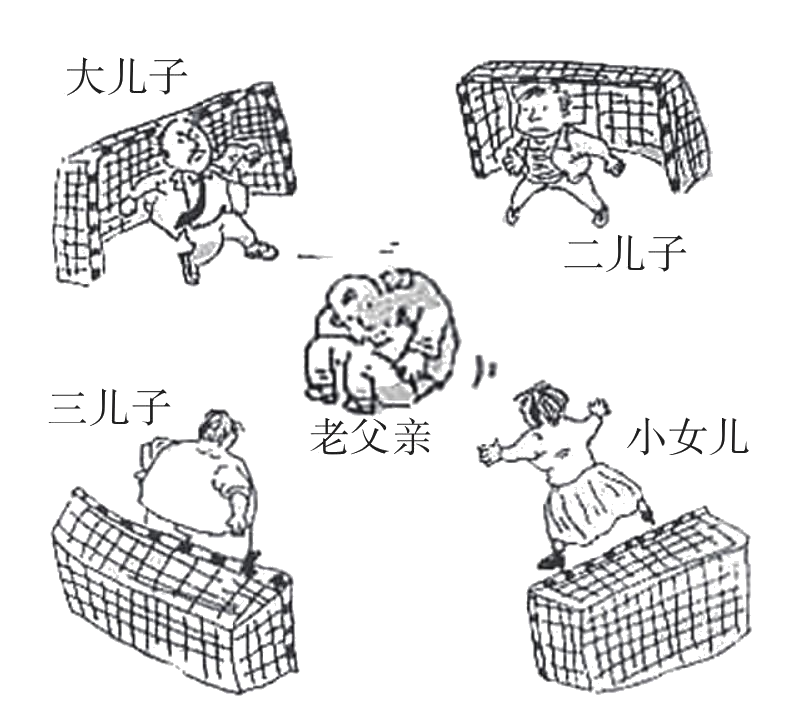
\includegraphics[width=0.56\linewidth]{picture/2005.png}
	\caption*{养老“足球赛”}
\end{figure}


\checkpagenumber




